%%%%%%%%%%%%%%%%%%%%%%%%%%%%%%%%%%%%%%%%%%%%%%%%%%%%%%%%%%%%%%%%%%%%%%%%%%%%%%%%
%science.tex: Chapter on DM physics:
%%%%%%%%%%%%%%%%%%%%%%%%%%%%%%%%%%%%%%%%%%%%%%%%%%%%%%%%%%%%%%%%%%%%%%%%%%%%%%%%
\chapter{Dark Matter}
\label{chapter:dm}
%%%%%%%%%%%%%%%%%%%%%%%%%%%%%%%%%%%%%%%%%%%%%%%%%%%%%%%%%%%%%%%%%%%%%%%%%%%%%%%%

Many physicists throughout history have been puzzled by new phenomena, but the confusion
surrounding dark matter -- estimated to be roughly 85\% of the total matter in the universe -- is
surely one of the biggest puzzles. While many astronomical observations at various scales have
confirmed the existence of dark matter, we have yet seen any observations of its particle
interacting with our detectors. This has ruled out many models for dark matter's particle nature,
but there are still many more available which can both explain the current observations of dark
matter gravitational and cosmological effects while skirt the limitations defined by the
\emph{lack} of observation in particle experiments.

\section{Dark Matter?}
As mentioned earlier, we physicists are a lazy bunch. Instead of referring to these phenomena
(\cref{sec:dm:evidence}) with a more accurate description, we invented a new term for our community
to refer to it. ``Matter'' originates from comparison to the particles that make ourselves up and
with which we are familiar -- both interact gravitationally, attracting other groups of ``matter''
into complex cosmological systems. The adjective ``dark'' refers to the literal fact that we cannot
see it with our telescopes. Other matter out in the universe can be seen via the light\footnote{
  Technically, I should say ``electromagnetic radiation'' since some observations use non-visible
  wavelengths (e.g. radio waves) to make observations of the cosmos, but that technicality gets in
  the way of motivating the ``dark'' adjective. } that it gives off (or reflects), so the fact that
this matter \emph{is not} visible in this way motivates the adjective.

That is it. \gls{dm-full} is merely a shorthand for this unknown aspect of the universe.

\section{Evidence for Dark Matter}
\label{sec:dm:evidence}

The first evidence physicists had for an unseen material floating throughout the universe was the
observation of galactic rotation curves \cite{rubin-rotationcurve-1980,rotationcurve-2000}. These
observations measure the speed of different stars within a galaxy and compare this speed to the
distance of that star from the center of the galaxy. We can calculate this relationship using
\gls{gr} \cite{rotationcurve-predictions-2007} and the observations differ drastically from this
calculation. The stars within galaxies we've observed move much faster than \gls{gr} would predict
(\cref{fig:rotation-curve}) leaving us with two explanations: either \gls{gr} is not the correct
theory to use in this situation or there is more un-seen mass floating within the galaxy allowing
these stars to move faster without leaving the galactic orbit.

Other indirect measurements give us additional ways to access information about this odd phenomena.
Within the framework of \gls{gr}, since energy and mass actually warp the fabric of spacetime, we
expect to see light itself follow a bent path around massive objects - a phenomenum that is called
\gls{grav-lens} and is observed and well modeled by \gls{gr}'s predictions \cite{gravlensing-2004}.
The accuracy of \gls{gr} within this context - a mass and distance scale similar to the rotation
curve oddities also observed - put more requirements on any modified theory of gravity that could
both explain the rotation curves and gravitational lensing. Additionally, measurements on some of
the largest scales and from the early universe display signs of a certain mass density attributed
to non-baryonic matter. \todo{bullet cluster figure}

The \gls{cmb} and \gls{bao} provide a method for deducing densities of various classes of matter in
the early universe. Gravity attracts while pressure from the squeezing of the plasma repules which
produces oscillations in the density of matter in space and time. These \gls{bao} are imprinted on
our snapshot of this early-universe plasma, the \gls{cmb}, which we can measure with a high degree
of accuracy and fit to various models of what existed at this time of the universe. The best fit of
these models corresponds to only $\sim 5\%$ of the mass density being normal matter like we see
today while the rest is composed of material that only significantly interacts gravitationally
\cite{planck-cmb-2015}.

\begin{itemize}
  \item Astronomy observations show lots of measurements
        \begin{itemize}
          \item Type1a Supernovae \cite{type1a-supernova-2010}
          \item Big Bang Nucleosynthesis \cite{nucleosynthesis-1998}
          \item Probably not mini black holes \cite{constraints-primordial-black-holes-2021}
        \end{itemize}
  \item Can conclude pretty comfortably that DM exists
\end{itemize}

\begin{figure}
  \centering
  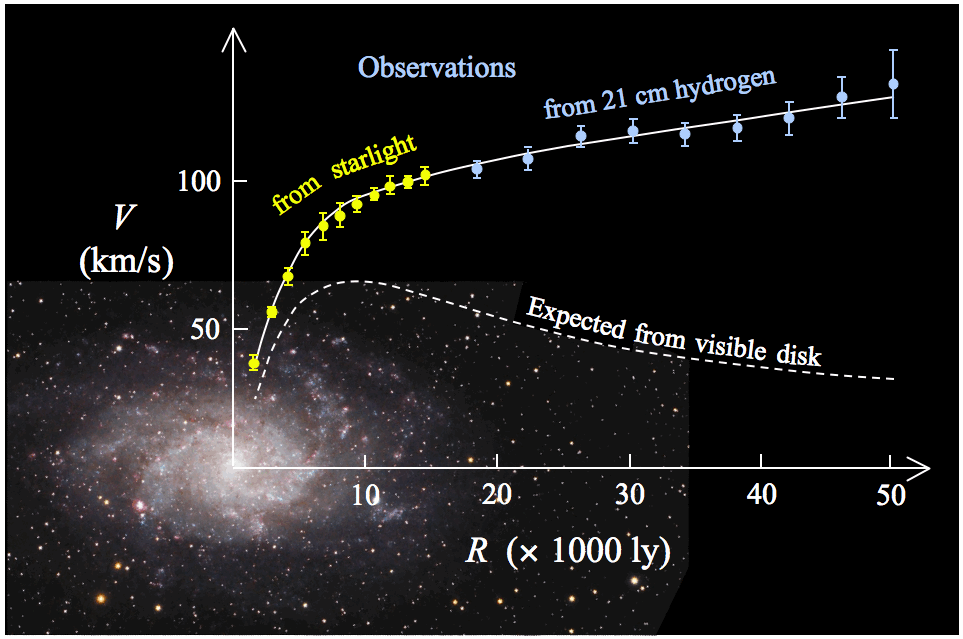
\includegraphics[width=0.6\textwidth]{figures/theory/rotation-curve-evidence-for-dm.png}
  \caption{
    Depiction of the velocity of stars within a galaxy as a function of their distance
    from the galactic center. The dotted line is a prediction of this relationship using
    \gls{gr} along with the mass tabulated from the visible starts while the data points
    (and the solid line fitted to them) are what are actually seen in galaxies today.
  }
  \label{fig:rotation-curve}
\end{figure}

\section{Particle Nature of Dark Matter}
The theoretical possibilities explaining dark matter are broad \cite{darksectors-2016} even when
excluding ourselves to the assumption that the dark matter phenomenum is explained by the existence
of a dark matter particle since the start of the start of the universe alongside our normal matter
particles. Here, I will refer to this particular dark matter as \gls{dm} which, in general, needs
to satisfy the following requirements.
\begin{itemize}
  \item \textbf{Dark} There has been no detection of these particles via the light observed with our telescopes;
        therefore, the dark matter has to not interact via the electromagnetic force.
  \item \textbf{Long Living} Measurements of \gls{dm}'s mass density and presence agree across time
        (from as early as the \gls{cmb} era), so \gls{dm} needs to have a long lifetime.
  \item \textbf{Observable Here} Measurements of \gls{dm} agree across different points in space,
        so it must be observable here on earth in some terresterial experiment.
  \item \textbf{Thermal Relic} Both \gls{dm} and standard matter have similar
        cosmological densities, so we expect some interaction (even a weak one) should connect their
        origins to the early universe allowing both to exist from the Big Bang.
  \item \textbf{Universal Density} Since we can indirectly measure a \gls{dm} mass density on
        cosmological scales, we impose the requirement that any \gls{dm} model needs to allow for
        this density.
\end{itemize}
Even with these assumptions and the requirements they imply, there still exist a plethora of
theoretical models that can satisfy all of them.

The upside is that a thermal-relic assumption closely connects the mass of individual \gls{dm}
particles to the interaction strength it has with standard matter. In this assumption, the \gls{dm}
evolves along with the universe allowing its number density to follow the density of standard
matter until it becomes too sparse to annihilate with itself and is thus ``frozen'' at a specific
number density. Since this ``frozen'' density changes depending on how easy it is for the the
\gls{dm} to interact with standard matter, the ``frozen'' number density goes down as the
interaction strength increases (\cref{fig:number-density}). The additional requirement of the
observed astronomical \emph{mass} density connects the mass of individual \gls{dm} particles to
their interaction strength with standard matter.
\begin{equation*}
  m_\chi \leftrightarrow \text{observed mass density}
  \leftrightarrow \frac{dN}{dV} \leftrightarrow
  \text{thermal relic hypothesis} \leftrightarrow
  \langle\sigma v\rangle
\end{equation*}
This connection allows us to define strict ``thermal relic targets'' which can help be measuring
sticks for how well our experiments search for \gls{dm} (these targets will appear in plots later).

\begin{figure}
  \centering
  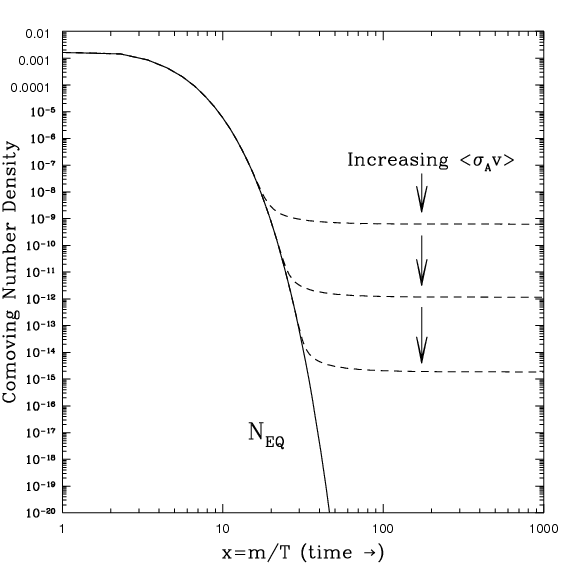
\includegraphics[width=0.5\textwidth]{figures/theory/number-density-at-freeze-out.png}
  \caption{
    From \cite{thermal-freezeout-diagram-1996}, the co-moving cosmological number density of \gls{dm} as a function of the universe
    temperature. As the universe cools, the number density decreases until the \gls{dm}
    becomes too sparse to interact with other \gls{dm} particles, ``freezing'' to a specific
    number density until today.
  }
  \label{fig:number-density}
\end{figure}

In addition to the connection between interaction strength and particle mass implied by the thermal
relic hypothesis, it also puts some loose bounds on mass of individual particles
(\cref{fig:dm-mass-scale}). If the mass is too low (approximately below the mass of the electron
$m_e$), then it is not feasible within our early-universe models to produce enough \gls{dm} to
match the observed \gls{dm} density currently frozen in. Similarly, if the mass is too high
($\gtrapprox 100~\text{TeV}$), the \gls{dm} will be too strongly coupled to the standard matter and
would be over-produced. \todo{Not sure about correctness of this.}

The mass scale of thermal relic \gls{dm} is further divided by the mass of the proton ($m_p$).
Above this threshold, the \gls{dm} could be interacting with standard matter through the standard
Weak Force (capital ``W'')\footnote{ The force already known to exist in nature which is
  responsible for phenomena like muon decay and nuclear fission. }; thus, they are named Weakly
Interacting Massing Particles (WIMPs). This phase space was first searched due to its theoretical
simplicitity: no new forces, just an extra particle (or two) creating the clouds of \gls{dm} we see
today. Unfortunately, these searches have not found evidence of a WIMP-like
signature\cite{supercdms-2018,damic-2020,xenon1t-2018} and the phase space has become tighter and
more exluded after many years of searching. Below this threshold, the \gls{dm} requires a new force
which also does not interact strongly with standard matter. In comparison to the heavier WIMPs,
this category of \gls{dm} is called ``Light'' \gls{dm}.

\begin{figure}
  \centering
  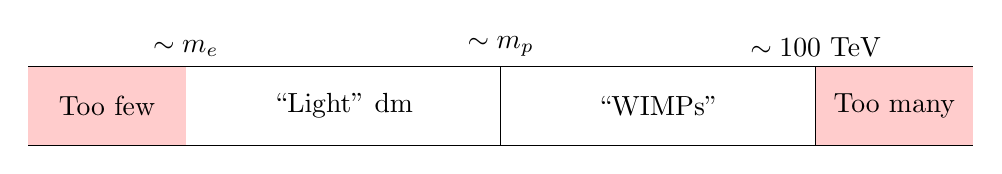
\begin{tikzpicture}
    % horizontal top/bottom lines
    \draw (0,0) -- (12,0);
    \draw (0,1) -- (12,1);
    % dividing lines along with relevant scale markers
    \draw (2,0) -- (2,1) node[above] {$\sim m_e$};
    \draw (6,0) -- (6,1) node[above] {$\sim m_p$};
    \draw (10,0) -- (10,1) node[above] {$\sim100~$TeV};
    % fill non-thermal ranges with light red
    \fill [red!20!white] (0,0) rectangle (2,1);
    \fill [red!20!white] (10,0) rectangle (12,1);
    % labels offering descriptions of ranges inside the boxes
    \node at (1,0.5) {Too few};
    \node at (4,0.5) {``Light'' \gls{dm}};
    \node at (8,0.5) {``WIMPs''};
    \node at (11,0.5) {Too many};
\end{tikzpicture}
  \caption{Mass scale of Thermal Relic \gls{dm}.
    The regions in red are excluded by applying the thermal relic assumption
    to our observations of the universe's early evolution.}
  \label{fig:dm-mass-scale}
\end{figure}

In general, the definition of a new force of nature is not well constrained; however, we can define
a ``baseline'' model that can represent more concrete theories in the context of our experiments.
For this situation, we postulate the existence of a massive gauge boson that represents an
additional $U_D(1)$ symmetry of nature. Since this additional symmetry has the same structure as
the electromagnetic interaction whose gauge boson is the standard photon, we generally refer to
this postulated massive boson as a \gls{dark-photon}. Without any additional assumptions, this new
\gls{dark-photon} does not interact with any standard matter, so we also assume that some
previously-unknown massive fields are able to interact with both. These other fields need to be
sufficiently massive (or sufficiently weakly coupled) so that they only allow the standard and dark
photons to weakly mix. \cref{fig:photon-mixing} diagrams how the standard and dark photons mix
which can then be effectively represented by a new vertex in our model.
\begin{equation*}
  \begin{tikzpicture}
    \begin{feynman}[inline]
      \vertex (dark) {\(A'\)};
      \vertex [right=of dark] (vtx);
      \vertex [above right=of vtx] (ellplus) {\(\ell^+\)};
      \vertex [below right=of vtx] (ellminus) {\(\ell^-\)};

      \diagram*{
      (dark) -- [photon] (vtx),
      (ellplus) -- [fermion] (vtx) -- [fermion] (ellminus),
      };
    \end{feynman}

    \node [right=of vtx] (eqn) {\(= i\epsilon g \gamma^\mu\)};
  \end{tikzpicture}
\end{equation*}
where the mixing strength $\epsilon$ encapsulates the effect of a massive field $\Phi$ at the energies
of our experiments (presumably low enough to avoid creation of a $\Phi$ directly).

\begin{figure}
  \centering
  \begin{tikzpicture}
    \begin{feynman}
      \vertex (standard) {\(\gamma\)};
      \vertex [right=of standard] (loopleft);
      \vertex [right=of loopleft] (loopright);
      \vertex [right=of loopright] (dark) {\(A'\)};

      \diagram*{
      (standard)
      -- [photon] (loopleft)
      -- [fermion, half left, edge label=\(\Phi\)] (loopright)
      -- [photon] (dark),
      (loopright)
      -- [fermion, half left, edge label=\(\Phi\)] (loopleft),
      };
    \end{feynman}
  \end{tikzpicture}
  \caption{Feynman diagram of how a massive field $\Phi$ could allow for a standard photon ($\gamma$)
    to mix with a dark photon ($A'$).}
  \label{fig:photon-mixing}
\end{figure}

\todo[inline]{Different methods of dark matter particle detection. Production is what we do here.}
This new vertex within our model for the universe enables a new process to occur: so-called
``Dark Bremsstrahlung'' (dark brem) where a charged particle exchanges a standard photon with
a nucleus and then emits a dark photon and recoils.

\begin{figure}
  \centering
  \begin{tikzpicture}
    \begin{feynman}
      \vertex (in) {\(\ell^-\)};
      \vertex [right=of in] (nuc);
      \vertex [below=of nuc, blob, label={below:\(Z\)}] (nucleus) {};
      \vertex [right=of nuc, dot] (emit);
      \vertex [above right=of emit] (recoil) {\(\ell^-\)};
      \vertex [below right=of emit] (decay) {\(A'\)};
      % \vertex [above right=of decay] (chi2) {\(\overline{\chi}\)};
      % \vertex [below right=of decay] (chi1) {\(\chi\)};

      \diagram*{
      (in) -- [fermion] (nuc) -- [fermion] (emit) -- [fermion] (recoil),
      (nucleus) -- [photon, edge label'=\(\gamma\)] (nuc),
      (emit) -- [photon] (decay),
      % (emit) -- [photon, edge label'=\(A'\)] (decay),
      % (chi2) -- [fermion] (decay) -- [fermion] (chi1),
      };
    \end{feynman}
  \end{tikzpicture}
  \caption{
    Feynman diagram for the dark brem process.
  }
  \label{fig:dark-brem-feynman}
\end{figure}

But what happens to the dark photon after it interacts with standard matter via this vertex? It
cannot be the long-lived \gls{dm} we view in the universe today because this vertex allows for it
to decay \emph{back} into standard matter pretty easily. This is where we expand on the idea of a
``dark sector''. In this description of \gls{dm}, we already have a dark photon representing some
force and a very heavy field that can interact with it. Suppose this ``dark sector'' also has other
particles (like the standard sector) -- one (or more) of which could be long-lived and represent
the \gls{dm} we observe in the universe today (so-called ``\gls{dm} candidates''). We can further
partition this category of models depending on what happens to the \gls{dark-photon} after we
produce it within an experiment.

\section{Invisible Signature}

One of the simplest options is to simply hypothesize another particle that can take on the role of
long-lived DM and only interact ``within'' this dark sector (i.e. it only interacts with the dark
photon from our point of view). Calling this particle $\chi$ (and its anti-particle
$\overline{\chi}$), we then have an additional dark sector vertex.
\begin{equation*}
  \begin{tikzpicture}
    \begin{feynman}[inline]
      \vertex (dark) {\(A'\)};
      \vertex [right=of dark] (vtx);
      \vertex [above right=of vtx] (ellplus) {\(\overline{\chi}\)};
      \vertex [below right=of vtx] (ellminus) {\(\chi\)};

      \diagram*{
      (dark) -- [photon] (vtx),
      (ellplus) -- [fermion] (vtx) -- [fermion] (ellminus),
      };
    \end{feynman}

    \node [right=of vtx] (eqn) {\(= i\alpha_{D} \gamma^\mu\)};
  \end{tikzpicture}
\end{equation*}
If the mass of the dark photon is greater than twice the mass of the $\chi$ ($m_{A'} > 2m_\chi$),
then this vertex can occur immediately after a dark photon is produced within an experiment.
Since the $\chi$ does not interact with our normal (standard model) particles, the energy
they have is ``lost'' from our perspective. \cref{part:ldmx} focuses on a proposed experiment
designed to precisely measure all of the \emph{visible} energy so that this ``invisible signature''
of DM being produced could be observed.

\section{Visible Signature}
There is no a priori reason for $m_{A'} > 2 m_\chi$, so we must accomodate the possiblity that
$m_{A'} < 2 m_\chi$. In this case, there would be a significant probability that the dark photon,
after it is produced, would convert \emph{back} into standard model particles. Since these decay
products are observable by our detectors, this signature is visible.

These visible signatures have a bit more complexity due to the fact that both a production process
and a decay process need to occur according to the model for DM we are testing. With this in mind,
many models that provide more detail about how particles exist within a dark sector have been
created, each of which providing a specific estimate for production and decay rates.
\cref{part:hps} focuses on an experiment looking for these visible signatures and my work
specifically was investigating some of these more intricate dark sector models in detail.
\cref{sec:theory-simps} and \cref{sec:theory-idm} provide more detail on the dark sector models
studied in this work.

\begin{itemize}
  \item Motivations for complicated model
        \begin{itemize}
          \item Direct detection is hard with LDM \cite{ldmconstraints-2019}
          \item super-WIMPs at keV mass scale \cite{superwimps-2008}
          \item iDM is interesting for others as well \cite{darkseaquest-2018}
        \end{itemize}
\end{itemize}

\subsection{Inelastic Dark Matter}
\label{sec:theory-idm}

One slightly more complicated extension simply proposes the existence of two more dark fermions:
\(\chi_2\) and \(\chi_1\) instead of just the \(\chi\). There is no reason for the DM to only
consist of one type of particle and indeed our standard matter is made up of several types of
particles (mostly three). The introduction of multiple fermions produces more complexity within the
dark sector, specifically enabling production and decay chains that, while still visible within
many of our experiments, would not follow the distribution or the rate described by the more
simplistic single-dark-fermion model. \cref{fig:dark-brem-idm-decay} shows a Feynman diagram of
dark brem production of the dark photon followed by its decay back into an electron-positron
pair which could be observed within a detector.

\begin{figure}
  \centering
  \begin{tikzpicture}
    \begin{feynman}
      \vertex (a) {$e^{-}$};
      \vertex [right= of a](d);
      \vertex [below=of d, blob,label={below:$Z$}] (e) {};
      \vertex [right= of d] (b);
      \vertex [above right= of b] (g) {$e^{-}$};
      \vertex [below right= of b] (aprime_decay);
      \vertex [below right= of aprime_decay] (rhod_decay);
      \vertex [above right= of aprime_decay] (dm) {$\chi_1$};
      \vertex [above right= of rhod_decay] (dm2) {$\chi_1$};
      \vertex [below right= of rhod_decay] (i);
      \vertex [above right= of i] (j) {$e^{-}$};
      \vertex [below right= of i] (k) {$e^{+}$};
      \diagram*[large] {
      (a) -- [fermion] (d),
      (d) -- [boson] (e),
      (d) -- [fermion] (b),
      (b) -- [fermion] (g),
      (b) -- [boson, edge label={$A'$}] (aprime_decay) -- [double, edge label={$\chi_2$}] (rhod_decay),
      (aprime_decay) -- [scalar] (dm),
      (rhod_decay) -- [scalar] (dm2),
      (rhod_decay) -- [boson, edge label={$A'^*$}] (i),
      (k) -- [fermion] (i) -- [fermion] (j),
      };
    \end{feynman}
  \end{tikzpicture}
  \caption{
    Diagram of dark brem production of a dark photon followed by its decay back into an electron-positron pair.
    The details of the $A'-\chi_2-\chi_1$ vertex are kept general and here are left as effective vertices.
  }
  \label{fig:dark-brem-idm-decay}
\end{figure}

\subsection{Strongly Interacting Massive Particles}
\label{sec:theory-simps}

%%%%%%%%%%%%%%%%%%%%%%%%%%%%%%%%%%%%%%%%%%%%%%%%%%%%%%%%%%%%%%%%%%%%%%%%%%%%%%%%
